\documentclass[document.tex]{subfiles}
\begin{document}
\chapter{Wyniki badań doświadczalnych \\ implementacji algorytmu Viterbiego}
\indent Do określenia poprawności działania opracowanej metody detekcji linii, 
wykorzystano zdjęcia z różnym poziomem zaszumienia. W celu porównania szybkości
działania poszczególnych implementacji algorytmu zdefiniowano zestaw zdjęć testowych
o różnym rozmiarze. Do przedstawienia wyników zestawień parametrów algorytmu Viterbiego
dla różnych wersji implementacji, została napisana funkcja automatycznie generująca plik .csv,
zawierający tabelę z parametrami wejściowymi oraz zestawienie szybkości przetwarzania każdego zdjęcia.
Na podstawie otrzymanego pliku zostały stworzone wykresy wizualizujące i umożliwiające
analizę i wyciągnięcie wniosków z przeprowadzonych badań.

%wrzucić zdjęcia pokazujące przykładowe wyniki detekcji linii dla różnych rodzajów obrazu - 3
%zdjęcia z przed i po
\begin{figure}[h]
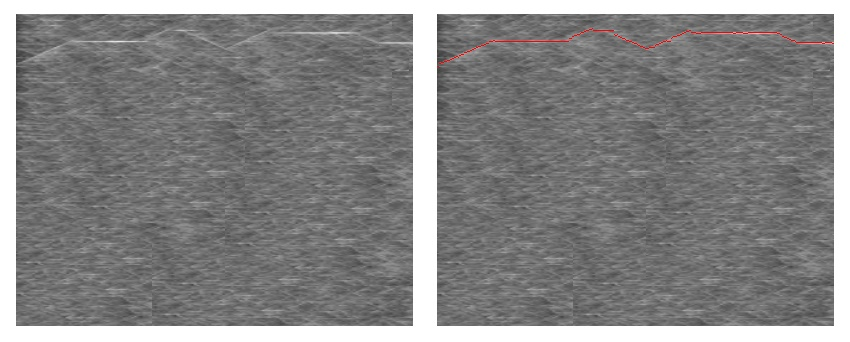
\includegraphics[scale=0.05]{detect_diff_0}
\caption{Przykład detekcji linii za pomocą algorytmu przedstawionego w rozdziale \ref{viterbi_line}}
\label{fig:sample_detect_0}
\end{figure}

\clearpage

\begin{figure}[h]
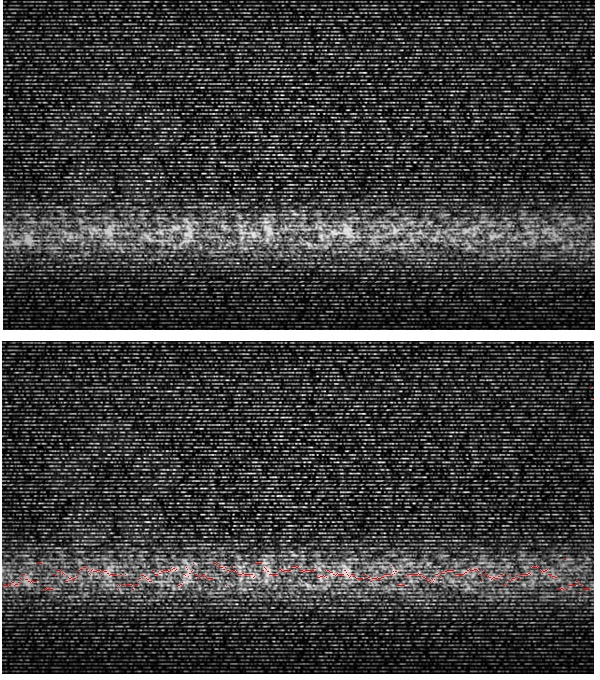
\includegraphics[scale=0.05]{detect_diff_1}
\caption{Przykład detekcji linii za pomocą algorytmu przedstawionego w rozdziale \ref{viterbi_line}}
\label{fig:sample_detect_1}
\end{figure}

\section{Porównanie czasu działania dla implementacji szeregowej, wielowątkowej
oraz z wykorzystaniem biblioteki OpenCL}
\indent W celu przetestowania szybkości opracowanego algorytmu wykorzystującego
kartę graficzną, porównano go z trzema innymi implementacjami algorytmu Viterbiego opisanymi
w rozdziale \ref{viterbi_chapter}.
W celu bardziej wymagającej oceny implementacji na GPU względem algorytmów wykorzystujących wyłącznie CPU, dodano
do flag kompilatora opcję \code{-O2} w celu włączenia optymalizacji programu.
Dzięki temu zaobserwowano diametralny wzrost szybkości wykonywania tych algorytmów.
\\
\indent Algorytmy były porównywane na podstawie szybkości przetwarzania zdjęć
w zależności od ich rozmiaru oraz zakresu lokalnego sąsiedztwa $g\in \langle g_l, g_h \rangle$
(patrz rozdział \ref{viterbi_line}).

%tu wrzucić wyniki z lapka
%tabela z wynikami

%napisac ze różnice w szybkości egzekucji pomiędzy kompilatorami w większości przypadków są pomijalnie małe
%dlatego nie jest rozpatrywane szybkość implementacji ze względu na rodzaj kompilatora

%wykresy


\section{Porównanie szybkości algorytmów dla różnych konfiguracji sprzętowych}
%porównać tu wyniki z pc'ta, dodać wykres porównujący średni
% czas wykonania algorytmu dla każdej z implementacji - nanieść/osobno wykres lapka i wykres pc'ta


\end{document}